\section{Evaluations}
\label{evaluation}

In this section, we show the results of experimental evaluation of decentralized search. We first give an overview of the datasets and introduce the experiment settings of our evaluations. The quality of approximated path generated by decentralized search is evaluated in two aspects, the distance accuracy and the path diversity, in~\ref{eval_accuracy} and~\ref{eval_diversity} respectively. We then show both overhead of index in~\ref{eval_overhead}. The throughput of our query processing system is shown in~\ref{eval_throughput}. Finally, we show the scalability of our system in~\ref{eval_scalability}.

\subsection{Datasets}
\label{eval_datasets}

\begin{table}
		\vspace{-0.5cm}
		\caption{Datasets}
		%\vspace{2 mm}
		\label{table:datasets}
		\begin{threeparttable}
			\centering
			\begin{tabular}{c|cccc} \hline
				Dataset & Type & $|V_{wcc}|$ & $|E_{wcc}|$ & $\overline{\sigma}$ \\ \hline
				Wiki & Communication & 2.4M & 4.7M & 3.9 \\ 
				Skitter & Internet & 1.7M & 11.1M & 5.07 \\ 
				Livejournal & Social & 4.8M & 43.4M & 5.6 \\ 
				Hollywood & Collaboration & 1.1M & 56.3M & 3.83 \\ 
				Orkut & Social & 3M & 117M & 4.21 \\ 
				Sinaweibo & Social & 58.7M & 261.3M & 4.15 \\ 
				Webuk & Web & 39.3M & 796.4M & 7.45 \\ 
				Friendster & Social & 65M & 1.8B & 5.03 \\ \hline
			\end{tabular}
			\begin{tablenotes}
				\item Datasets with the number of vertices and edges in the largest WCC, and the average shortest distance $\overline{\sigma}$ of 100,000 vertex pairs.
			\end{tablenotes}
		\end{threeparttable}
		\vspace{-0.3cm}
\end{table}

We evaluate our algorithm on 8 complex networks from different disciplines collected from Snap~\cite{snapnets} and NetworkRepository~\cite{nr} as shown in table~\ref{table:datasets}. 
%All are complex networks that have power-law degree distributions and relatively small diameters. 
To simplify our experiments, we treat them as undirected, un-weighted graphs and only use the largest weakly connected component of each graph. 
%All datasets are collected from Snap~\cite{snapnets} and NetworkRepository~\cite{nr}.

\subsection{Experiment settings}
\label{eval_system}

We evaluate our algorithms in both distributed setting, 20 Amazon EC2 m4.xlarge nodes, and centralized setting, one Cloudlab~\cite{RicciEide:login14} c8220 server. 
Powergraph~\cite{180251} and Snap~\cite{snapnets} are used as platforms respectively. All algorithms are implemented in C++. 
%For the distributed setting, we use 20 Amazon EC2 m4.xlarge virtual machines, each has 4 vCPUs and 16 GB memory. For centralized version, we use a Cloudlab~\cite{RicciEide:login14} c8220 server with two 10-core 2.2GHz E5-2660 processors and 256GB memory. Powergraph~\cite{180251} and Snap~\cite{snapnets} are platforms for distributed version and centralized version respectively. All algorithms are implemented in C++. 

%The landmark selection strategy we use is a variation based on $DEGREE/h$~\cite{Potamias:2009:FSP:1645953.1646063}. When selecting a new landmark, each vertex receives a rank that is the product of its degree and the sum of distances to all the existing landmarks. The vertex with the highest rank will be a new landmark.

We use $DEGREE/h$ proposed in~\cite{Potamias:2009:FSP:1645953.1646063} as our landmark selection strategy. We randomly generate 100,000 queries by randomly choosing 1,000 vertices as source vertices and 100 target vertices for each source vertex as BFS is extremely slow for large graphs. 

\subsection{Approximation Accuracy}
\label{eval_accuracy}

\begin{figure*}[ht]
    \centering
    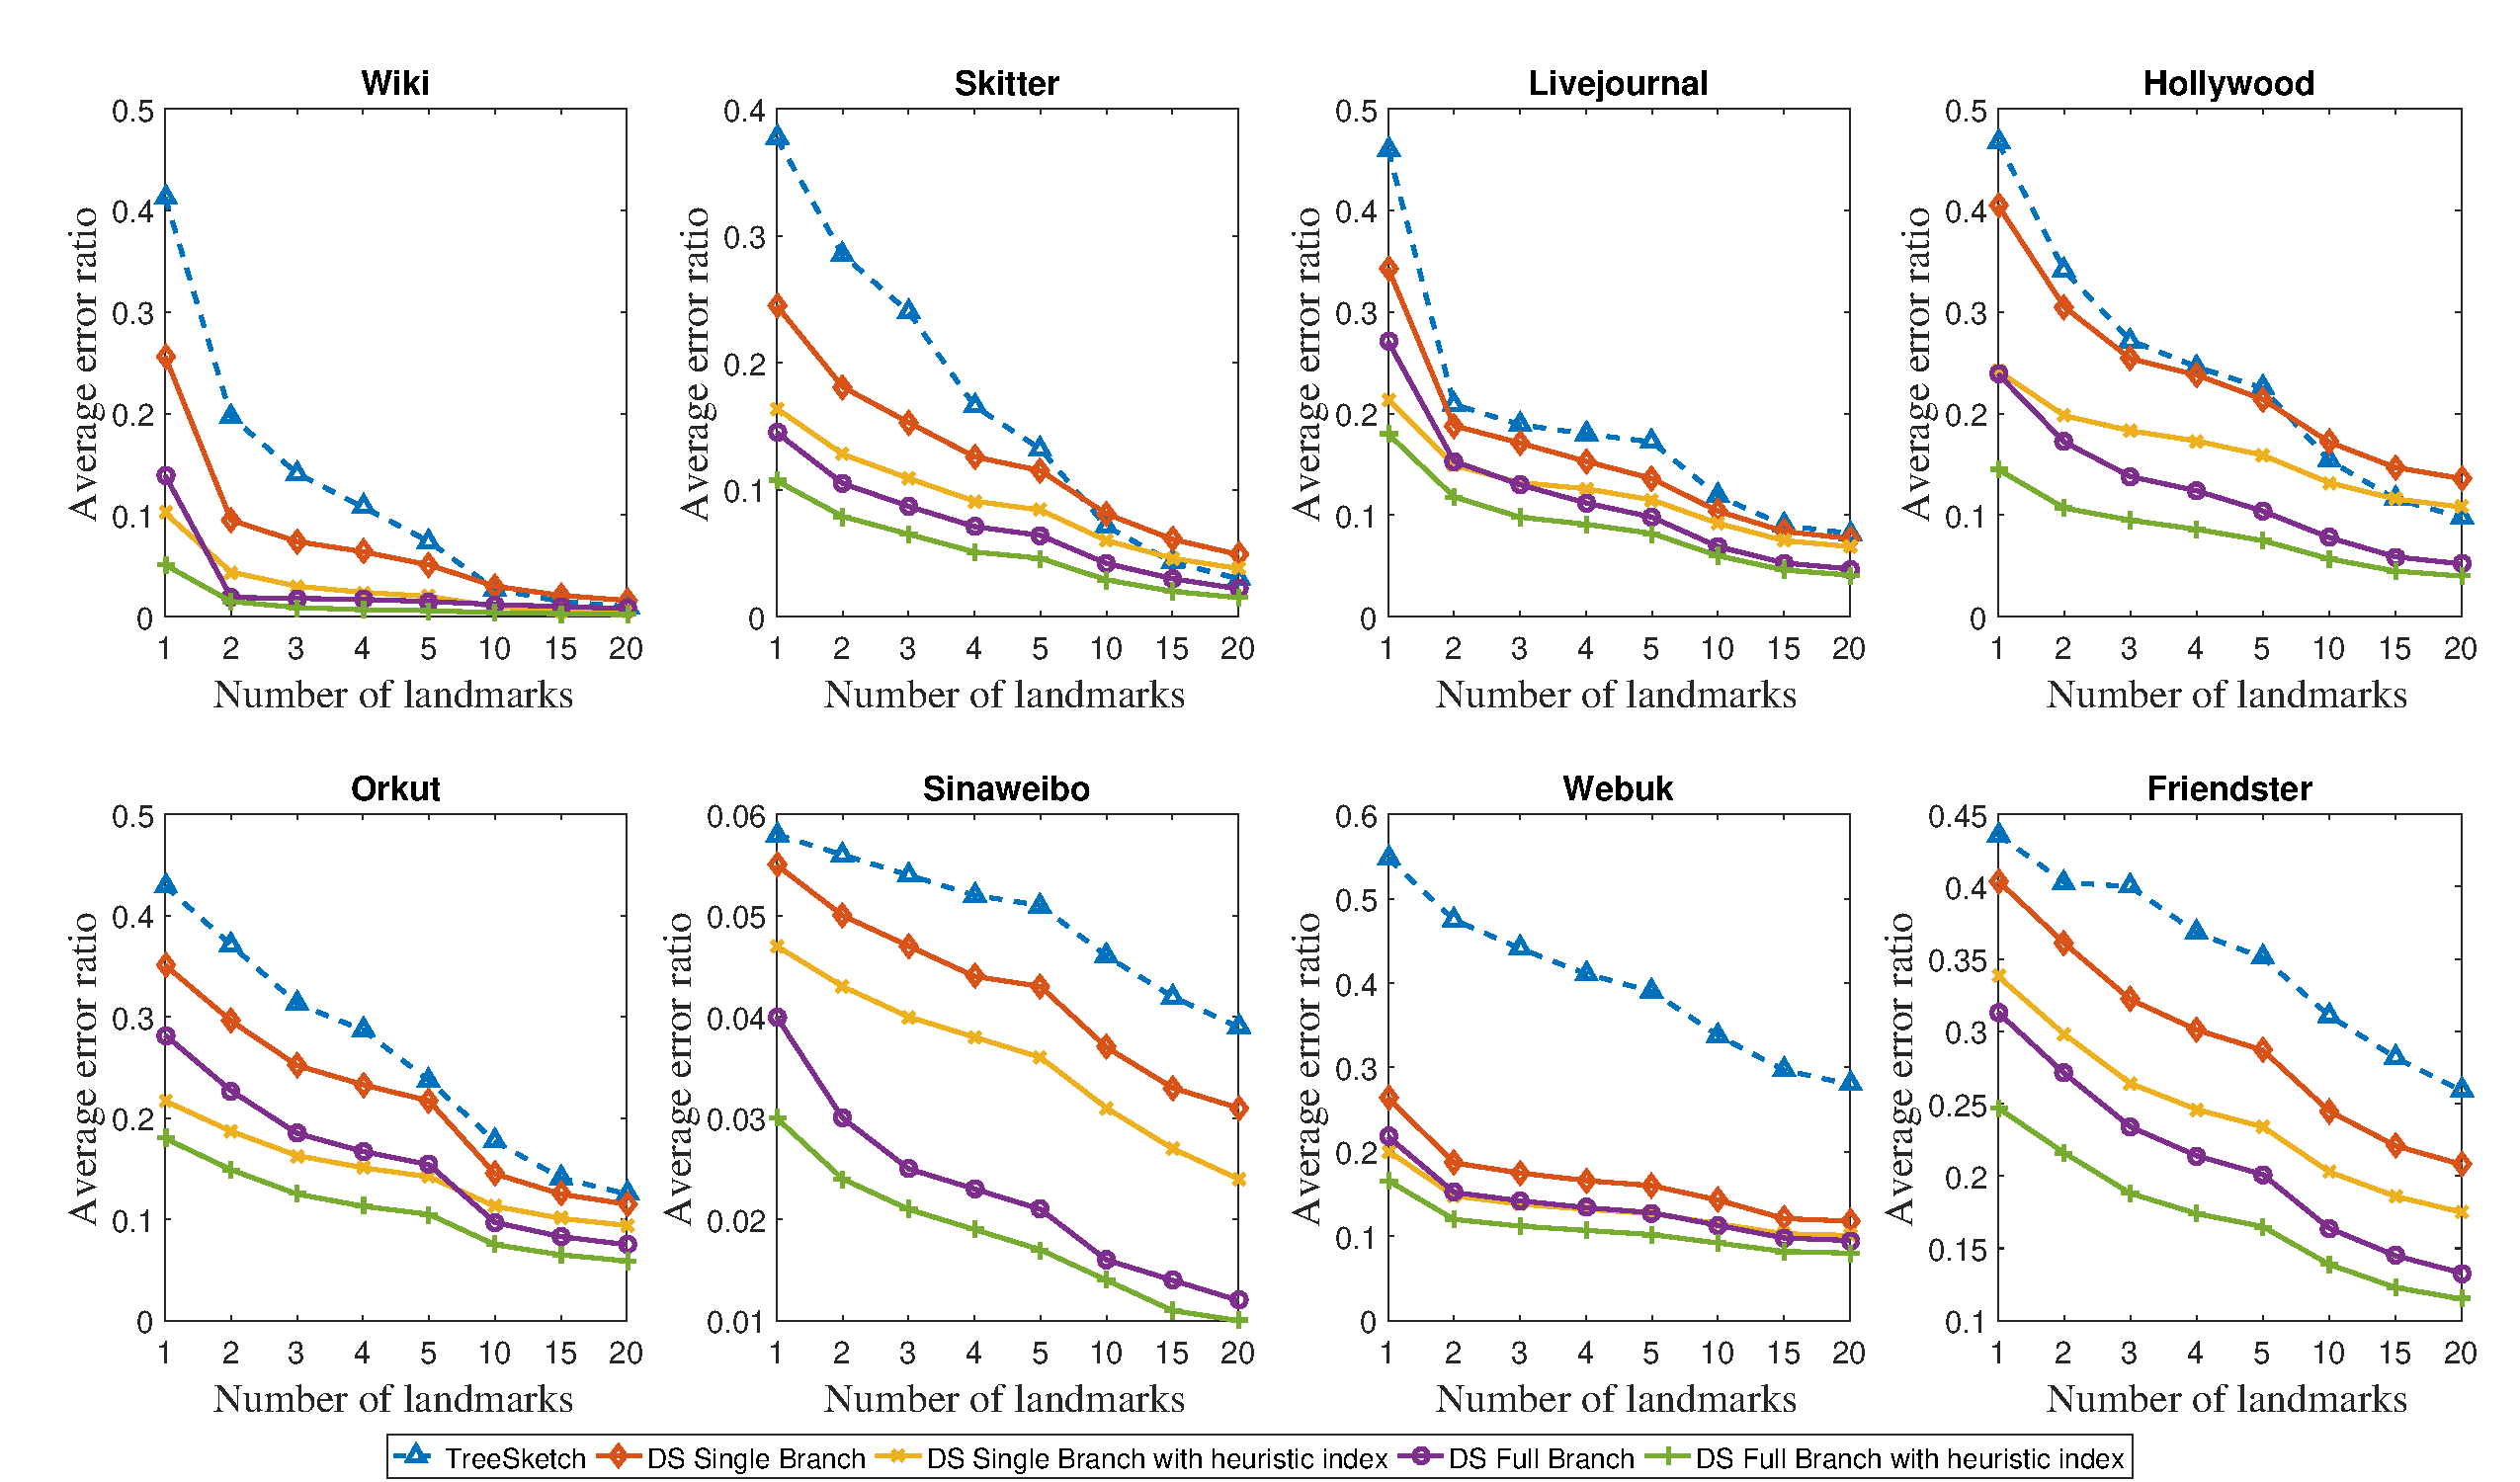
\includegraphics[width=\linewidth]{./figures/accuracy_stepy.pdf}
    \caption{The accuracy of the approximated distance of decentralized search compared to TreeSketch.}
    \label{fig:accuracy_stepy}
\end{figure*}

We first evaluate the approximation accuracy of the decentralized search. We use the average approximation error as the measure of accuracy which is defined as follows:
\[
E_{\tilde{p}(s,t)} = \frac{|\tilde{p}(s,t)| - d_G(s,t)}{d_G(s,t)}
\]
We show the results under various landmark set size of 4 variations of bidirectional decentralized search with mixture of different tie breaking strategies and index construction approach. We also list the results of a state-of-the-art online search approach, TreeSketch~\cite{Gubichev:2010:FAE:1871437.1871503}. Note that the online search in~\cite{6399472} is similar to TreeSketch with only different stop condition so we do not include it to the comparison. We run TreeSketch with random index construction strategy.

We can see in Fig.~\ref{fig:accuracy_stepy} that decentralized search achieves better accuracy in most of cases. Especially with small landmark sets, i.e. $k < 5$, decentralized search outperforms TreeSketch on all the graphs. When the full branch decentralized search are carried on the index constructed by our greedy heuristic, the performance gain is the most noticeable, with 43.3\% to 87.7\% lower average error ratio for 1 landmark and 50\% to 80\% lower average error ratio for 20 landmarks than TreeSketch on all graphs.

Full branch tie strategy always outperforms single branch tie strategy with large margins with same landmark sets. The average error ratio shown in Fig.~\ref{fig:accuracy_stepy} of full branch decentralized search with regular index is 17.4\% to 45.7\% lower than single branch decentralized search for 1 landmark and 19.5\% to 61.8\% lower with 20 landmarks on various graphs. As the number of landmark increases, the accuracy gain increases.   

Decentralized search carried on index constructed by greedy heuristic has lower error ratio than decentralized search with regular index. The average error ratio shown in Fig.~\ref{fig:accuracy_stepy} is 14.5\% to 60.2\% lower for single branch and 21.1\% to 63.3\% lower for full branch for 1 landmark. For 20 landmarks, the search is 10.4\% to 68.8\% lower for single branch and 12.8\% to 75\% lower for full branch.

\subsection{Path Diversity}
\label{eval_diversity}

\begin{table}
	\vspace{-0.5cm}
	\caption{Path diversity (k = 2)}
	%\vspace{2 mm}
  \label{table:pdiv}
  \centering
  \begin{tabular}{c|ccc} \hline
		&Path cnt&Path cnt& \\
		Graph&Decetralized Search&TreeSketch&$\overline{r_p}$ \\ \hline
		Wiki&28.9&1.9&0.372 \\ 
		Skitter&24.1&2.4&0.418 \\ 
		Livejournal&30.8&1.9&0.338 \\ 
		Hollywood&9.9&2.6&0.471 \\ 
		Orkut&19.2&3.2&0.465 \\ 
		Sinaweibo&32.0&3.0&0.301 \\ 
		Webuk&704.1&2.0&0.501 \\ 
		Friendster&16.8&2.8&0.39 \\ \hline
  \end{tabular}
	\vspace{-0.3cm}
\end{table}

We show in this section that decentralized search achieves better path diversity by finding more paths and not being constrained by the index. Table~\ref{table:pdiv} shows the average number of paths with shortest approximated distance returned by decentralized search with full branch tie strategies compared to TreeSketch. The average path count of full branch decentralized search is much higher than that of TreeSketch, from 3.73 to 345.13 times for various graphs.

Moreover, decentralized search is not restricted by labels of the source and the target vertices. We define the ratio $r_p$ as the number of vertices not in label source and target compared to total number of vertices except the source and target vertex:
\[
r_p(s,t) = \frac{|\{u:u \in p(s,t), u \notin L(s) \cup L(t)\}|}{|{v:v \in p(s,t), v \neq s, v \neq t}|}
\]
The higher the $r_p$'s value, the lower the dependence of a path to label of source and target vertices. As shown in Table~\ref{table:pdiv}, the average $r_p$ for full branch decentralized search on various graphs ranges from 0.301 to 0.501.

\subsection{Overhead}
\label{eval_overhead}

\begin{table}
		\caption{Space overhead}
		\vspace{2 mm}
    \label{table:ioh}
    \centering
    \begin{tabular}{c|cc} \hline
				&Index size&\\
				Graph&per landmark(MB)&Query size(B)\\ \hline
				Wiki&189.9&369.8 \\ 
				Skitter&143.7&412.9 \\ 
				Livejournal&429.4&419.9 \\ 
				Hollywood&84.1&377.5 \\ 
				Orkut&246.3&390.7 \\ 
				Sinaweibo&4313.8&367.4 \\ 
				Webuk&4068.9&506.5 \\ 
				Friendster&5497.7&437.7 \\ \hline
    \end{tabular}
\end{table}

The index and query overhead is shown in table~\ref{table:ioh}. In our implementation, both the label for each vertex and approximated paths are stored as vectors. And each vertex id is represented by 8-byte unsigned long. The size shown in table~\ref{table:ioh} is the sum of vector size of each vertex. 

\subsection{Throughput}
\label{eval_throughput}

\begin{figure*}[ht]
		\vspace{-0.5cm}
    \centering
    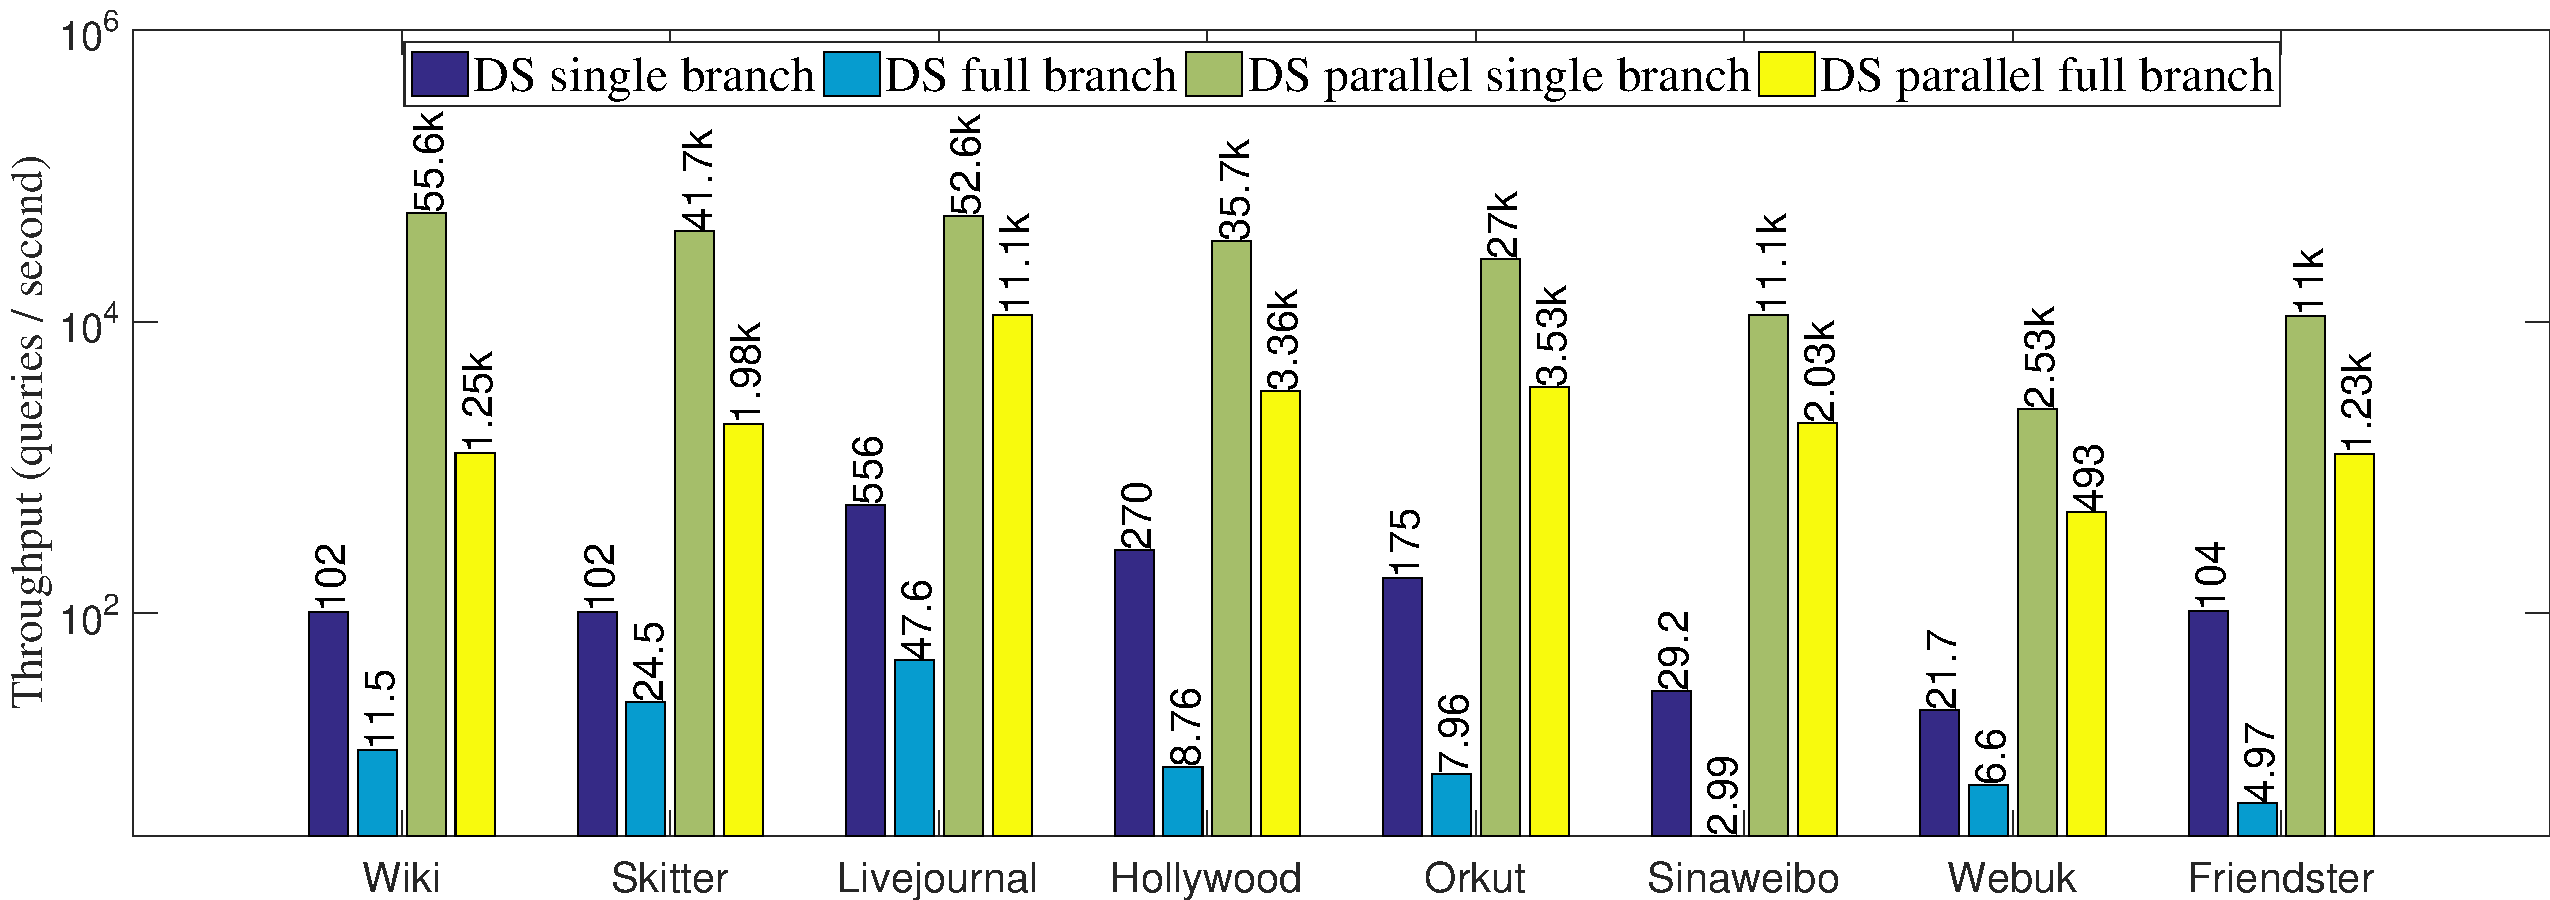
\includegraphics[width=0.95\linewidth]{./figures/throughput.pdf}
    \caption{The throughput of sequential and parallel version decentralized search.}
    \label{fig:throughput}
		\vspace{-0.5cm}
\end{figure*}

Fig.~\ref{fig:throughput} shows the throughput of our system in log scale for both sequential mode and parallel mode. The throughput of parallel mode is calculated based on running 100,000 queries simultaneously. The throughput of the parallel mode is much higher than the sequential mode, from 94.7 to 544.4 times for single branch decentralized search and 74.7 to 679.1 times for full branch decentralized search. 

We can also see that due to the search duplicates itself for full branch decentralized search, the throughput is 3.2\% to 30.4\% of single branch for the sequential mode and 2.3\% to 21.1\% of single branch for the parallel mode. 

\subsection{Scalability}
\label{eval_scalability}

%\begin{figure}[ht]
    %\centering
    %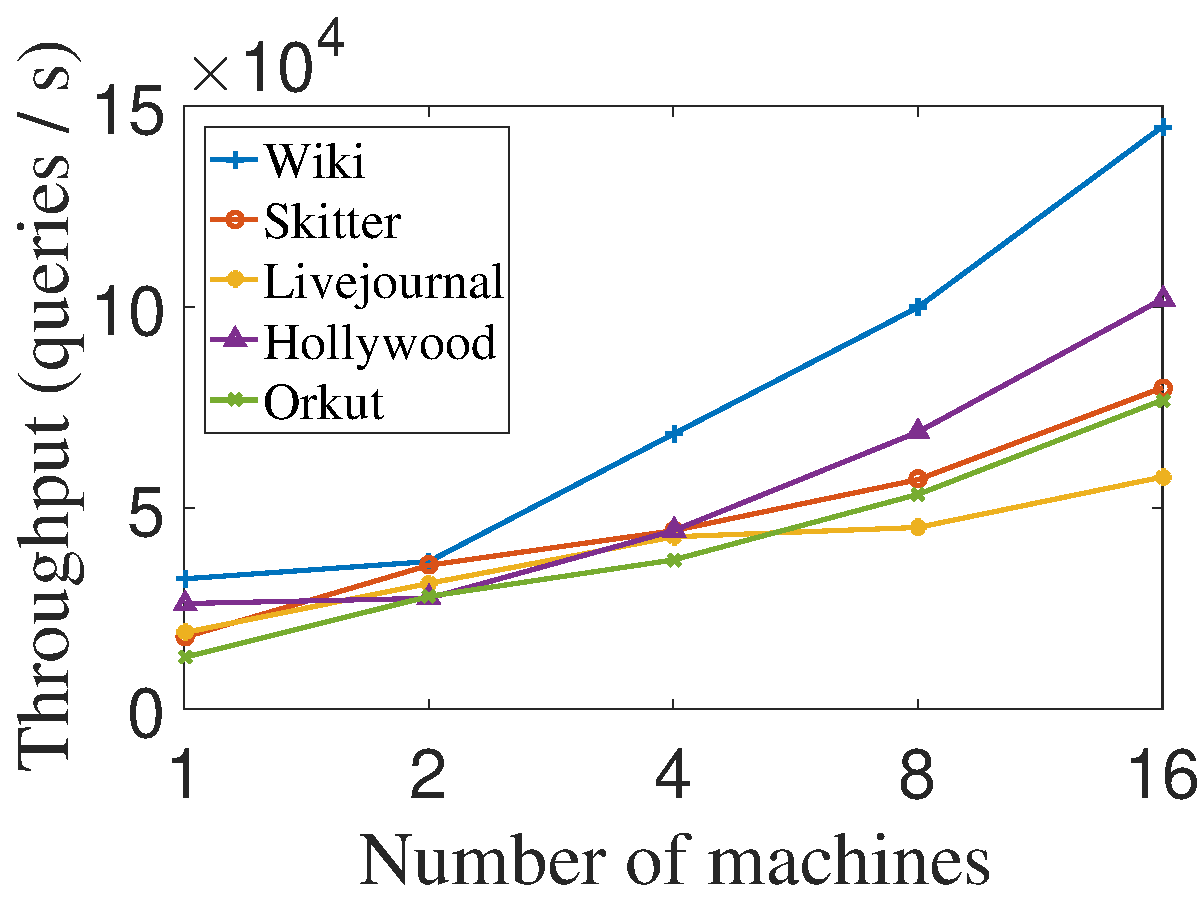
\includegraphics[width=\linewidth]{./figures/scale_machine_throughput.pdf}
    %\caption{The throughput as the number of machines increases with 1 millions queries running simultaneously}
    %\label{fig:scale_machine}
%\end{figure}
%
%\begin{figure}[ht]
    %\centering
    %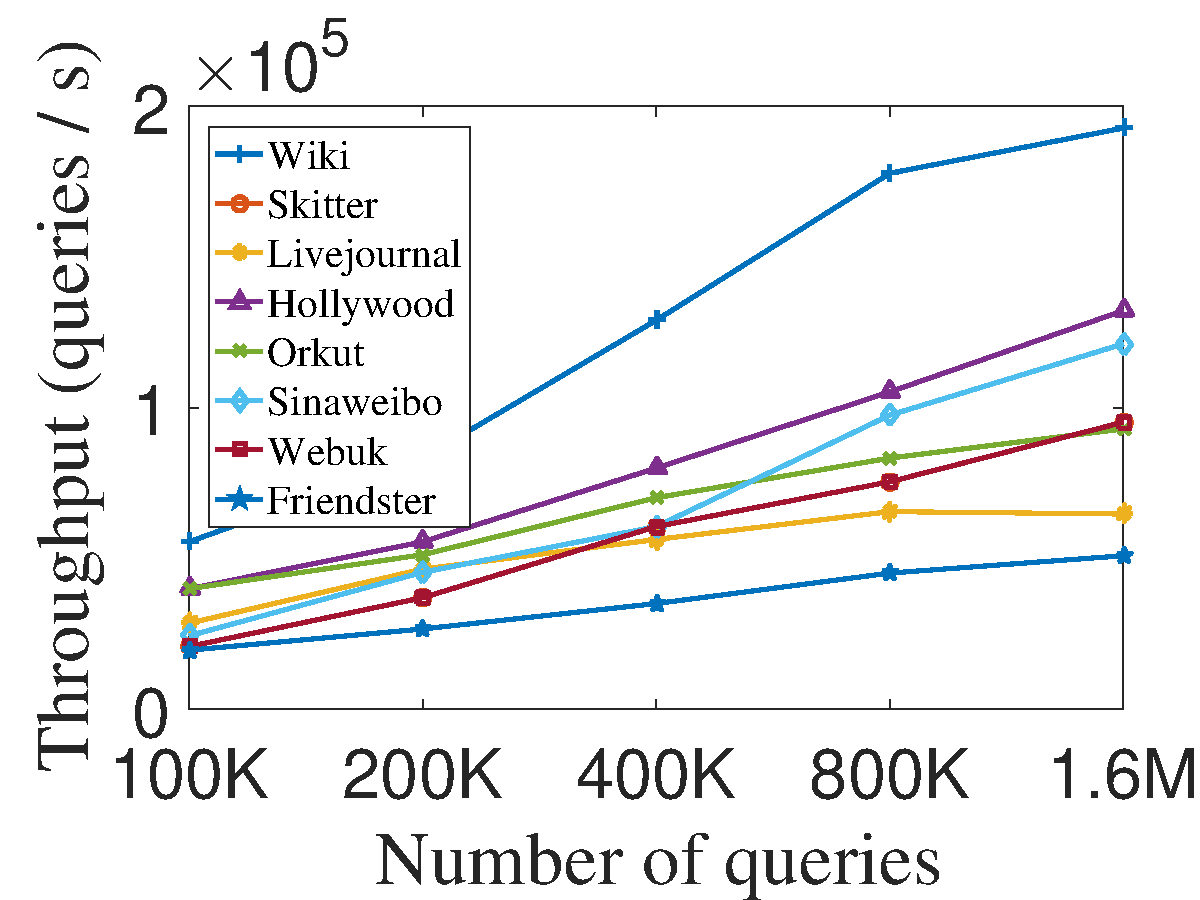
\includegraphics[width=\linewidth]{./figures/scale_query_throughput.pdf}
    %\caption{The throughput on 20 machines as the number of queries running simultaneously increases}
    %\label{fig:scale_query}
%\end{figure}

\begin{figure}[ht]
		\vspace{-0.2cm}
    \centering
    \subfigure[Number of machines increases 			\label{fig:scale_machine}]{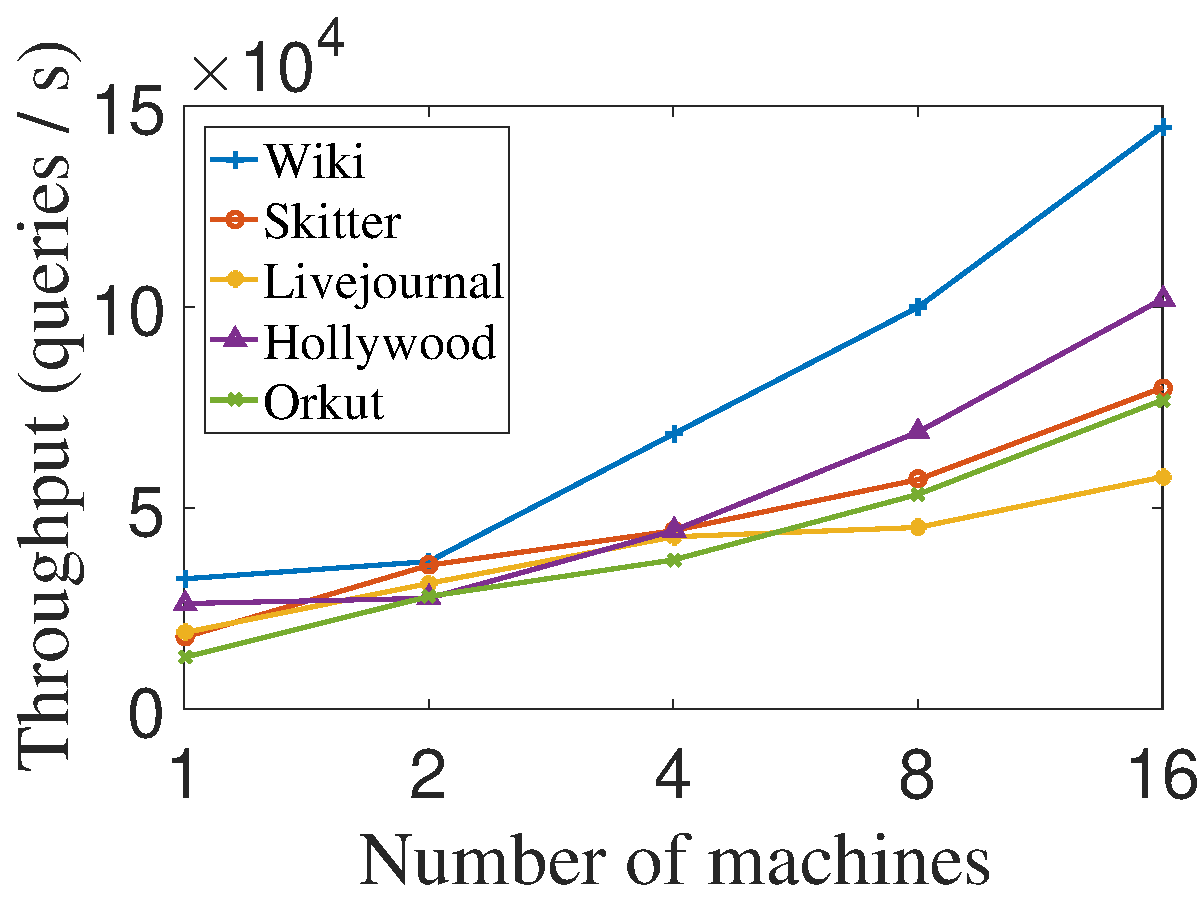
\includegraphics[width=0.24\textwidth]{./figures/scale_machine_throughput.pdf}}
    \subfigure[Number of queries increases \label{fig:scale_query}]{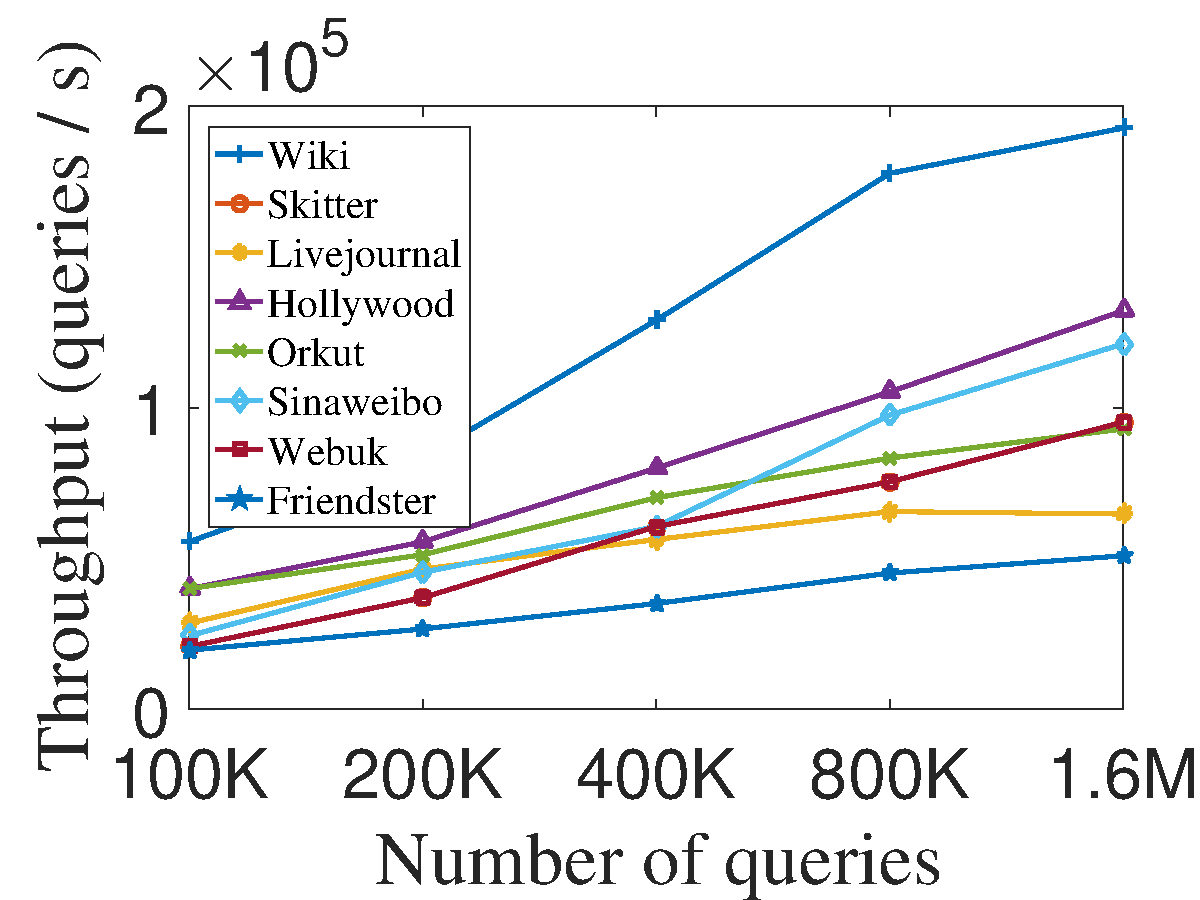
\includegraphics[width=0.24\textwidth]{./figures/scale_query_throughput.pdf}}
    \caption{Throughput of decentralized search}
\end{figure}

Since our algorithm is designed for large-scale networks, scalability is another major concern of our algorithm. We show how our algorithm performs as number of machines and queries increases. We only perform single branch decentralized search here as full branch search is equal to multiple independent single branch searches, thus have the similar trend.

We first evaluate the throughput as number of machines increases. Results shown in Fig.~\ref{fig:scale_machine} are based on the results of running 1,000,000 queries simultaneously. We can see the throughput increases as the number of machines increases. The throughput on 16 machines is 3.0 to 5.9 times higher than on a single machine for various graphs. Note that we do not have results for the 3 largest graphs as they are not able to fit into fewer than 8 machines.

We also show the trend of the throughput as number of queries running simultaneously increases. All the experiments are carried on 20 machines. We can see in Fig.~\ref{fig:scale_query} the constant growth of throughput as the number of queries running simultaneously increases. The growth of throughput slows down for large number of queries as the system limits are reached, i.e., memory size or network bandwidth. The throughput for 1,600,000 queries running simultaneously is 2.3 to 5.0 times higher than it for 100,000 queries.
